\chapter{Método Proposto}



% -.~.-.~.-.~.-.~.-.~.-.~.-.~.-.~.-.~.-.~.-.~.-
\section{Visão geral}

O método proposto divide-se nas seguintes etapas:

\missingfigure[figheight=100mm]{Diagrama do método}


% -.~.-.~.-.~.-.~.-.~.-.~.-.~.-.~.-.~.-.~.-.~.-
\section{Modelo do robô}

Nesta seção, são detalhados os procedimentos para representar o manipulador
robótico como um conjunto MBS e utilizá-lo para simular as trajetórias
referentes a uma determinada tarefa. O manipulador será descrito pelo conjunto
de Sistemas de Coordenadas (SC's) referente a cada uma de suas juntas, pelas
distâncias entre os SC's e posição dos centros de massa de cada elo, e pelos
parâmetros de massa e momento de inércia de cada elo. Os elos do robô e a
ferramenta acoplada no efetuador representam cada corpo do sistema MBS. A
modelagem do manipulador é simplificada utilizando as rotinas de CAS
desenvolvida especialmente para MBS, o Sophia, assim como a notação algébrica de
Lesser, apresentada na seção~\ref{sec::sophia-kane}.

\subsection{Descrição do braço robótico}

O manipulador escolhido para estudo é o mesmo que será utilizado no projeto EMMA
para revestimento de superfícies metálicas por HVOF. Trata-se de um robô
comercial modelo MH12, da série MOTOMAN, fabricado pela Yaskawa Motoman
(Figura~\ref{fig::mh12_foto}).

\begin{figure}[h]
    \centering
    \begin{subfigure}[b]{0.3\textwidth}
        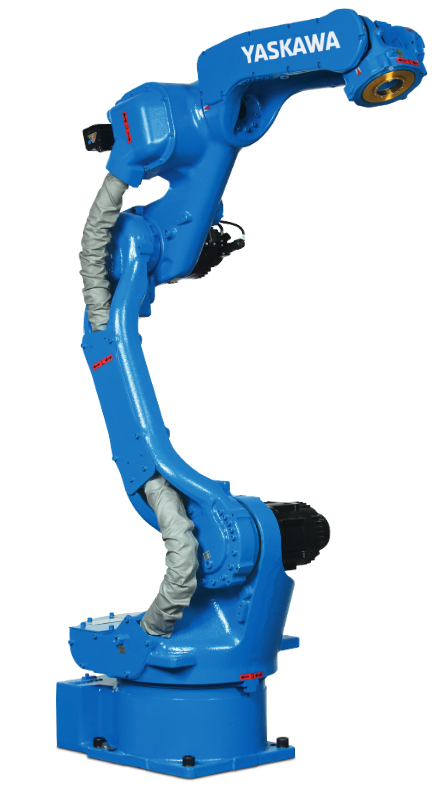
\includegraphics[width=\textwidth]{figs/mh12_foto}
        \caption{MOTOMAN MH12. \\Fonte: adaptada de}
        \label{fig::mh12_foto}
    \end{subfigure}
    \quad %add desired spacing between images, e. g. ~, \quad, \qquad, \hfill
    % etc.
      %(or a blank line to force the subfigure onto a new line)
    \begin{subfigure}[b]{0.5\textwidth}
        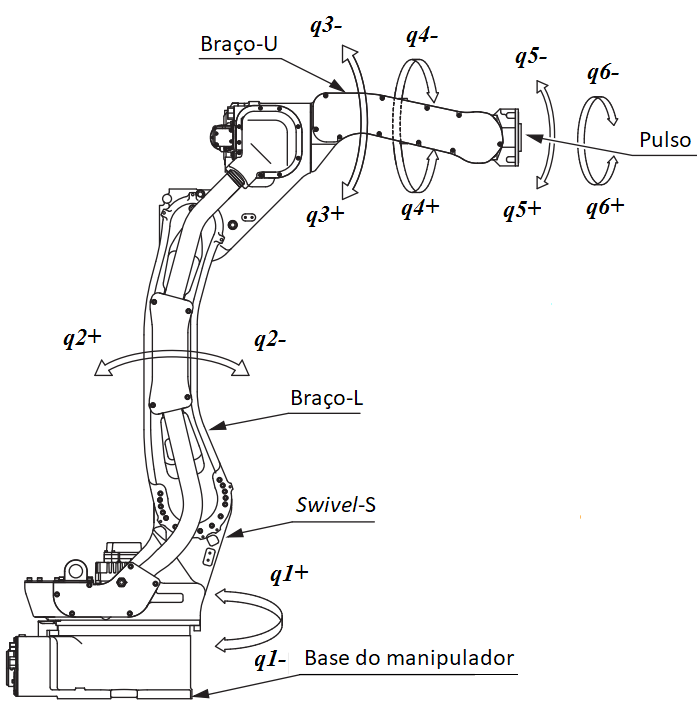
\includegraphics[width=\textwidth]{figs/mh12_diagram}
        \caption{Diagrama dos elos e juntas. \\Fonte: adaptada de}
        \label{fig::mh12_diagram}
    \end{subfigure}
    \caption{Manipulador robótico para modelo}\label{fig::resumo_mh12}
    \todo[inline]{Inncluir referências das figuras}
\end{figure}

\begin{table}[h]
\centering
\caption{Sistemas de coordenadas, elos e coordenadas generalizadas}
\label{tab::resumo_mh12}
\begin{tabular}{@{}clc@{}}
\toprule
SC & Elo              & \multicolumn{1}{l}{Coord. gen. associada} \\ \midrule
Z  & Pedestal do robô & -                                         \\
S  & \textit{Swivel}  & q1                                        \\
L  & Braço inferior   & q2                                        \\
U  & Braço superior   & q3                                        \\
R  & Braço de rolagem & q4                                        \\
B  & Pulso            & q5                                        \\
T  & Efetuador        & q6                                        \\ \bottomrule
\end{tabular}
\end{table}

Este robô é um braço antropomórfico de 6 juntas rotacionais e 6 graus de
liberdade (6 gdl), contendo o último elo um porta-ferramentas que suporta uma
carga útil de até 12 kg. A Figura~\ref{fig::mh12_diagram} apresenta os nomes dos
elos e coordenadas generalizadas associados a cada um dos sistemas de
coordenadas e também aparecem em resumo na Tabela~\ref{tab::resumo_mh12}.

O alcance horizontal deste manipulador chega a 1,440~m, e vertical a
2,511~m. Estão representados no diagrama do espaço de trabalho na
Figura~\ref{fig::workspace} em que a área sombreada é formada por todos os
pontos alcançáveis pelo manipulador, dentro dos limites de cada junta.

\begin{figure}[h]
	\centering 
 	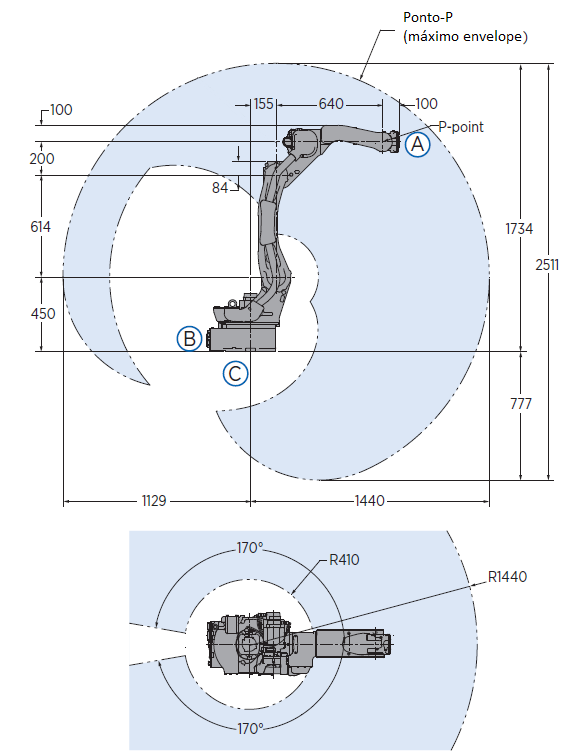
\includegraphics[width=0.7\textwidth]{figs/workspace}
 	\caption{Vistas lateral e superior do espaço de trabalho. \\Fonte: adaptada
 	de}
 		\todo[inline]{Inncluir referência da figura}
 	\label{fig::workspace}
\end{figure}

Conforme discutido na seção~\ref{sec::manind}, este tipo de braço robótico
permite desacoplar o sistema em 2 problemas: posicionamento e orientação. Logo,
para simplificar o modelo e o cálculo da cinemática inversa, serão consideradas
as 3 primeiras juntas para posicionamento e 3 últimas (pulso esférico) para
orientação da ferramenta.

A última junta, no efetuador, tem a finalidade de orientar a ferramenta em torno
do seu eixo axial. Como o processo de revestimento por HVOF independe desta
orientação, esta junta não será incluída, mantendo este acoplamento rígido, o
que transforma os dois últimos elos em apenas um corpo.
Como resultado, tem-se um sistema de 5 gdl.


\subsection{Cinemática Direta}

\subsection{Dinâmica}

\subsection{Cinemática Inversa}

\subsection{Tarefa e trajetória}

\subsection{Modelo teórico MBS -- Robô}


% -.~.-.~.-.~.-.~.-.~.-.~.-.~.-.~.-.~.-.~.-.~.-
\section{Modelo da base}

\subsection{Geometria e CAD}

\subsection{Matriz de Rigidez}

\subsection{Matriz de Amortecimento}

\subsection{Análise Elementos Finitos}

\subsection{Modelo teórico MBS -- Base}


% -.~.-.~.-.~.-.~.-.~.-.~.-.~.-.~.-.~.-.~.-.~.-
\section{Ensaio Experimental}

\subsection{Bancada experimental}

\subsection{Programas de aquisição dos dados experimentais}

\subsection{Tratamento dos dados}

\subsection{Cálculo dos parâmetros modais da estrutura}


% -.~.-.~.-.~.-.~.-.~.-.~.-.~.-.~.-.~.-.~.-.~.-
\section{Modelo acoplado robô e base}

\subsection{Base rígida}

\subsection{Base flexível}


% -.~.-.~.-.~.-.~.-.~.-.~.-.~.-.~.-.~.-.~.-.~.-
\section{Estudos de casos para avaliação do método}

\subsection{Trajetórias do efetuador}

\subsection{Base rígida}

\subsection{Base de testes}

\subsection{Base modular PRP}

\subsection{Base com pouca rigidez}
